\paragraph*{}
Data compression is a set of steps for packing data into a smaller space, while allowing for the original data to be seen again. Compression is a two-way process: a compression algorithm can be used to make a data package smaller, but it can also be run the other way, to decompress the package into its original form. Data compression is useful in computing to save disk space, or to reduce the bandwidth used when sending data (e.g., over the Internet).
\begin{figure}[h!]
\centering
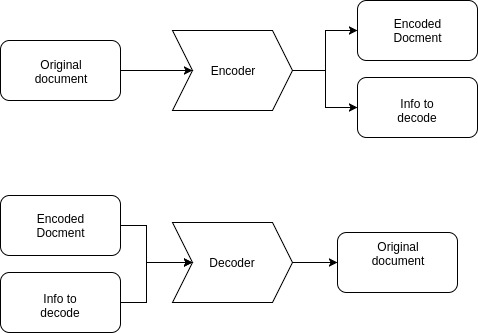
\includegraphics[width=0.7\linewidth]{images/flow_chart.jpg}
\caption{The flow chart show how data can be compressed and decompressed.}
\end{figure}
\paragraph*{}
Compression can be either lossy or lossless. No information is lost in lossless compression. Lossy compression reduces bits by removing unnecessary or less important information.
\paragraph*{Two main goals of this projects are:}
\begin{enumerate}
\item Implements three lossless compression algorithms (run length, shannon-fano and jpeg) on real life data to see how it really works on different kinds of data.
\item Build a simple web application to work on the Internet environment for practice. 
\end{enumerate}

